%##########################  CHAPER 6: APPLICATION  #######################

\chapter{Entwicklung der Anwendung}\label{kap:application}

Dieses Kapitel beschreibt die Realisierung der Anwendung 
als autonomes Kamera System zur, 
Wildtiererkennung, welches auf einem Raspberry Pi 4 läuft.

Dabei wird es neben der Implementierung der Inferenz für eines der 
traininierten Modelle, auch um die Auswahl einer 
nachtsichtgeeigneten Kamera und der implementierung 
einer Kommunikationsmöglichkeit zur übermittlung 
der Daten gehen.



%-------------------------  SECTION 1: AUFBAU  ------------------------
\section{Hardware}\label{sec:aufbau}


Der Aufbau der Anwendung besteht aus einem Raspberry Pi 4, auf dem 
der Programmcode läuft, sowie dem Neural Compute Stick 2
für die Inferenz, welcher über eine USB Schnittstelle
mit dem Raspberry Pi verbunden wird.

Zur aufnahme der Bilder wurde ein Raspberry Pi Kamera Modul mit 
5MP OV5647 Sensor der Marke Longrunner verwendet.
Dieses ermöglicht durch mechanisches zu und abschalten eines Infrarot 
Filters vor die Linse zwischen Tag und Nachtsicht zu wechseln.
Der dafür verwendete Magnetschalter wird dabei über einen 
Helligkeitsensor getriggert.
Im Infrarotmodus befindet sich der Filter nicht 
vor der Linse, wodurch neben den elektromagnetischen 
Wellen des Sichtbaren Lichts auch die etwas langwelligeren 
(850nm) des Infrarot Spektrums auf die Linse treffen und 
verarbeitet werden können.

Zudem verfügt die Kamera über zwei Infrarot LEDs, 
sodass auch Aufnahmen bis zu 3m Entfernung
in völliger Dunkelheit gemacht werden können. Diese haben 
den vorteil gegenüber normalen Scheinwerfern, 
das die Tiere von keiner Sichtbaren Lichtquelle 
gestört oder verscheucht werden.
verbunden wird das Kamera Modul über die CSI 
(Camera Serial Interface) 
Schnittstelle des Raspberry Pi's.
\vspace{1cm}



%https://www.amazon.de/gp/product/B07R4JH2ZV/ref=ppx_yo_dt_b_asin_title_o01_s00?ie=UTF8&psc=1


\begin{minipage}{0.55\textwidth}
    \centering
    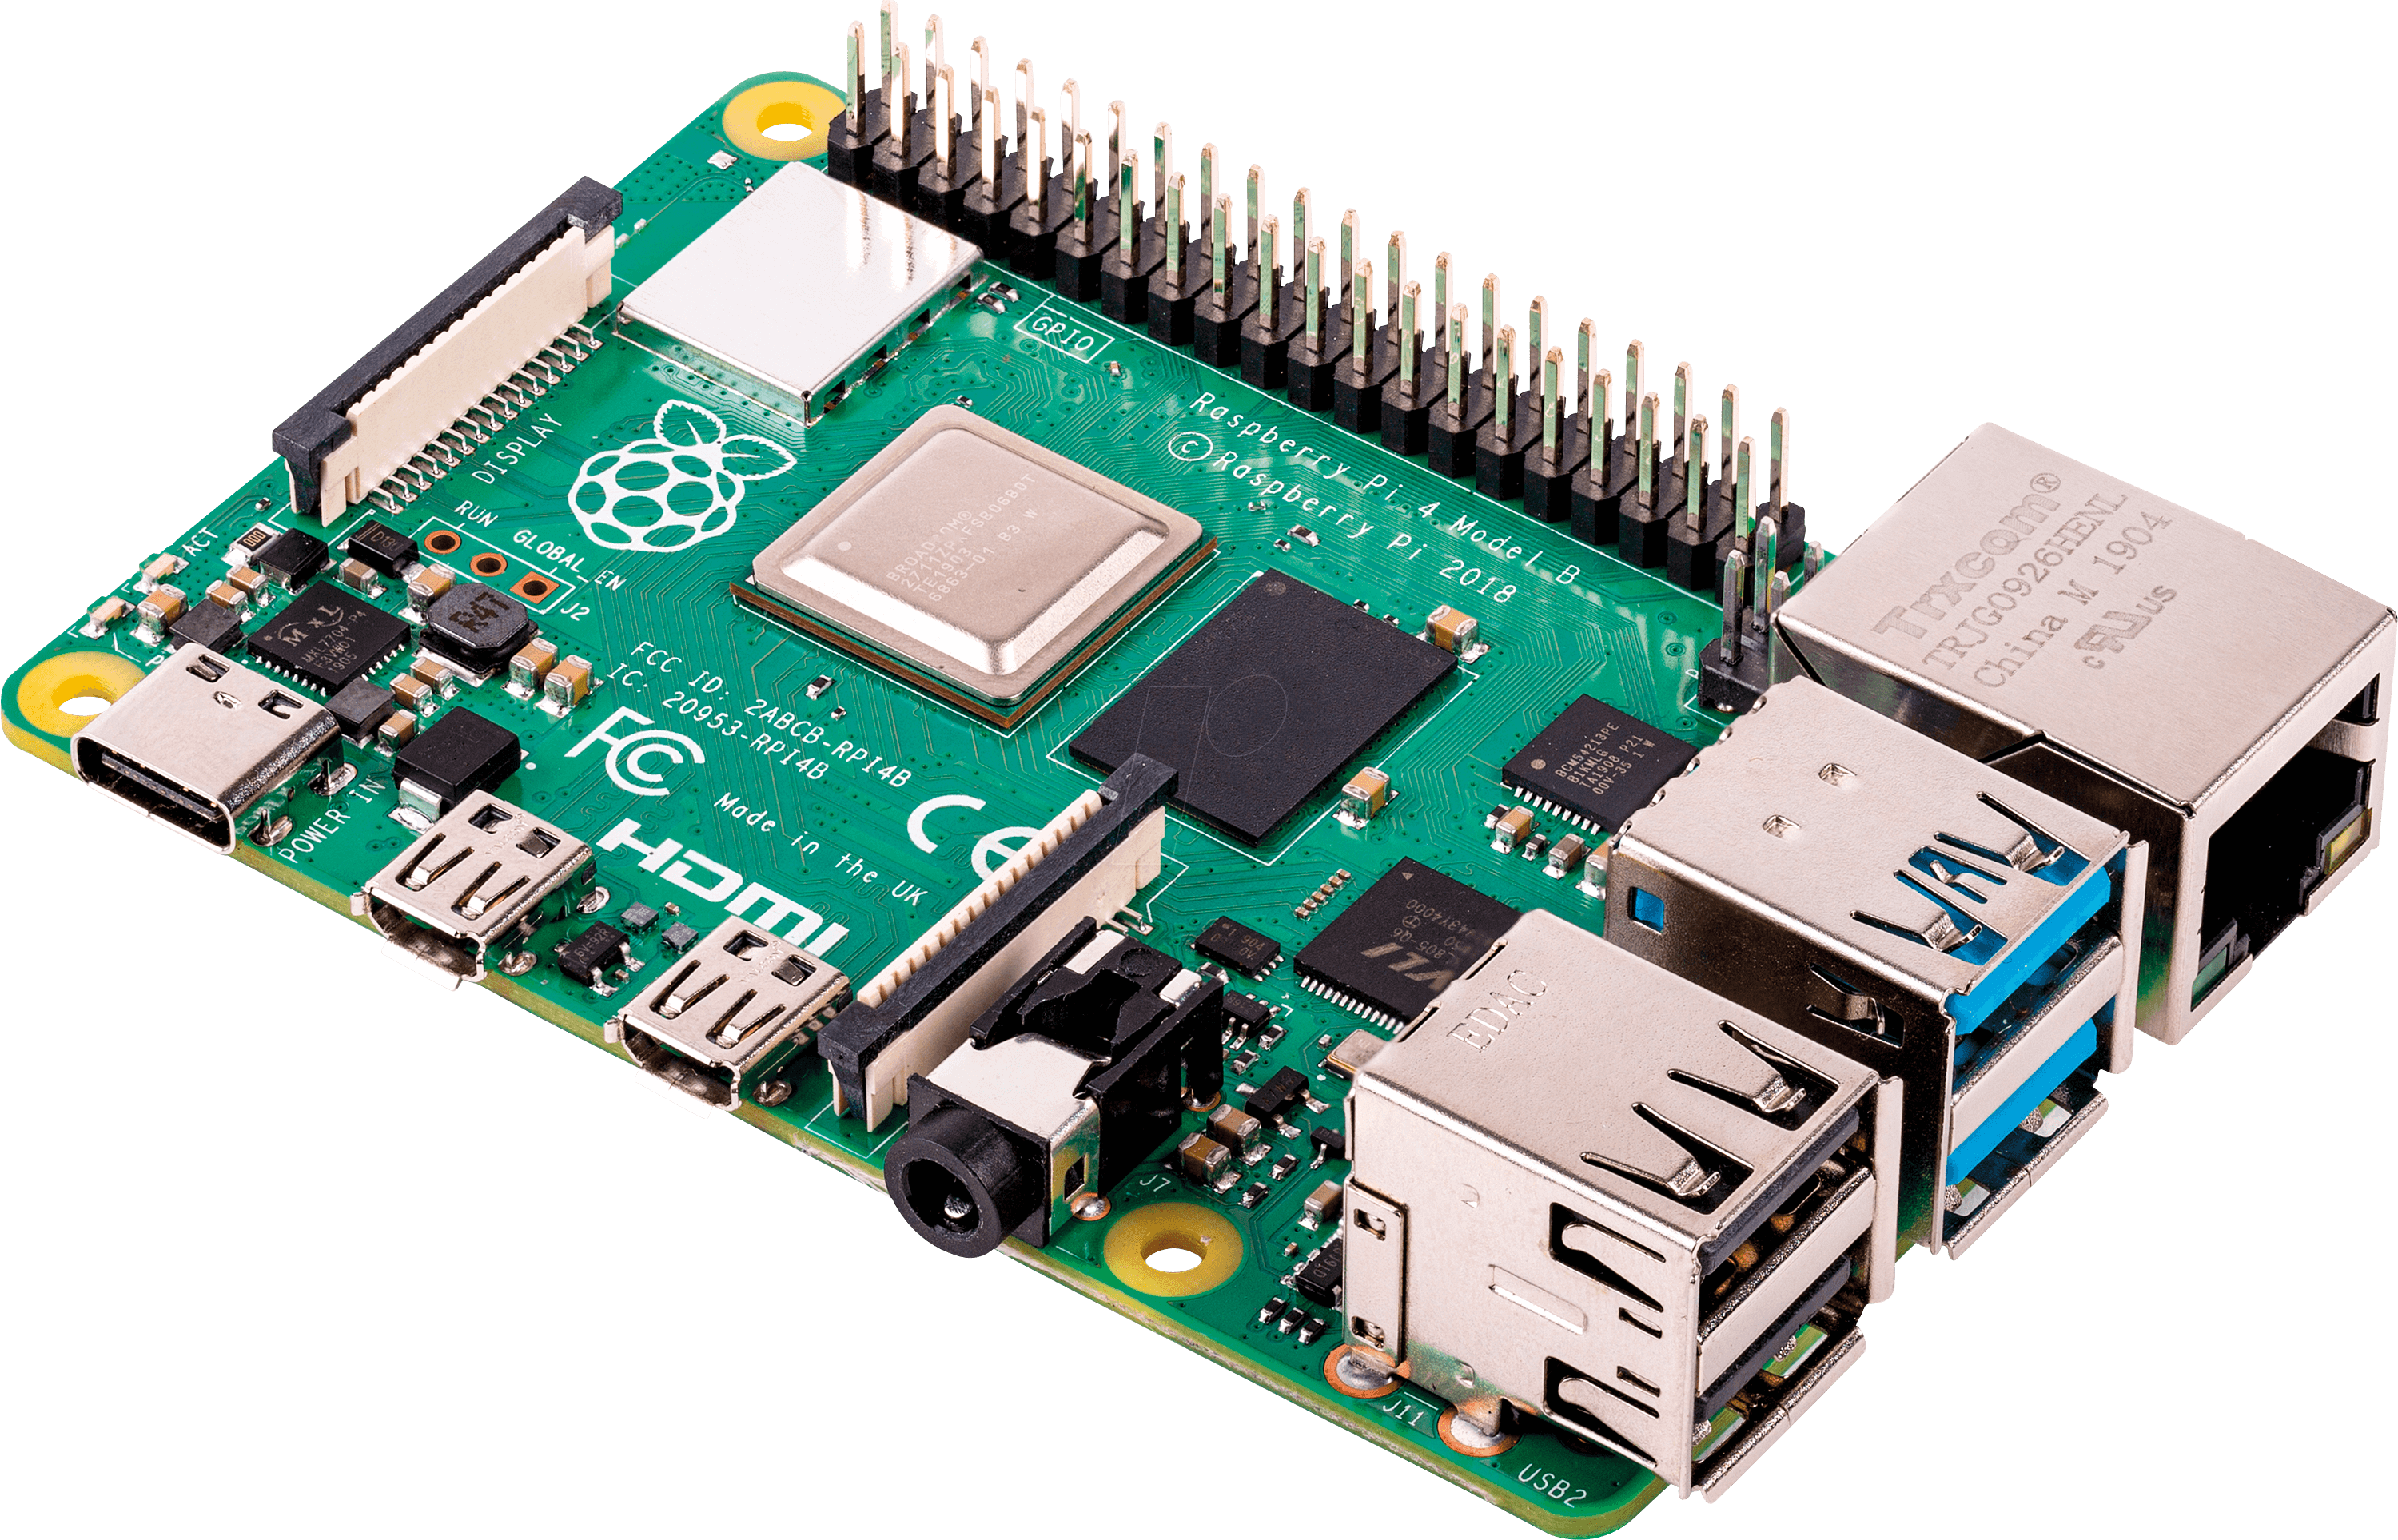
\includegraphics[width=0.8\textwidth]{./Bilder/raspberrypi_4.png}
    \captionof{figure}{Raspberry Pi 4}
    \label{img:raspberrypi}
\end{minipage}
\begin{minipage}{0.45\textwidth}
    \centering
    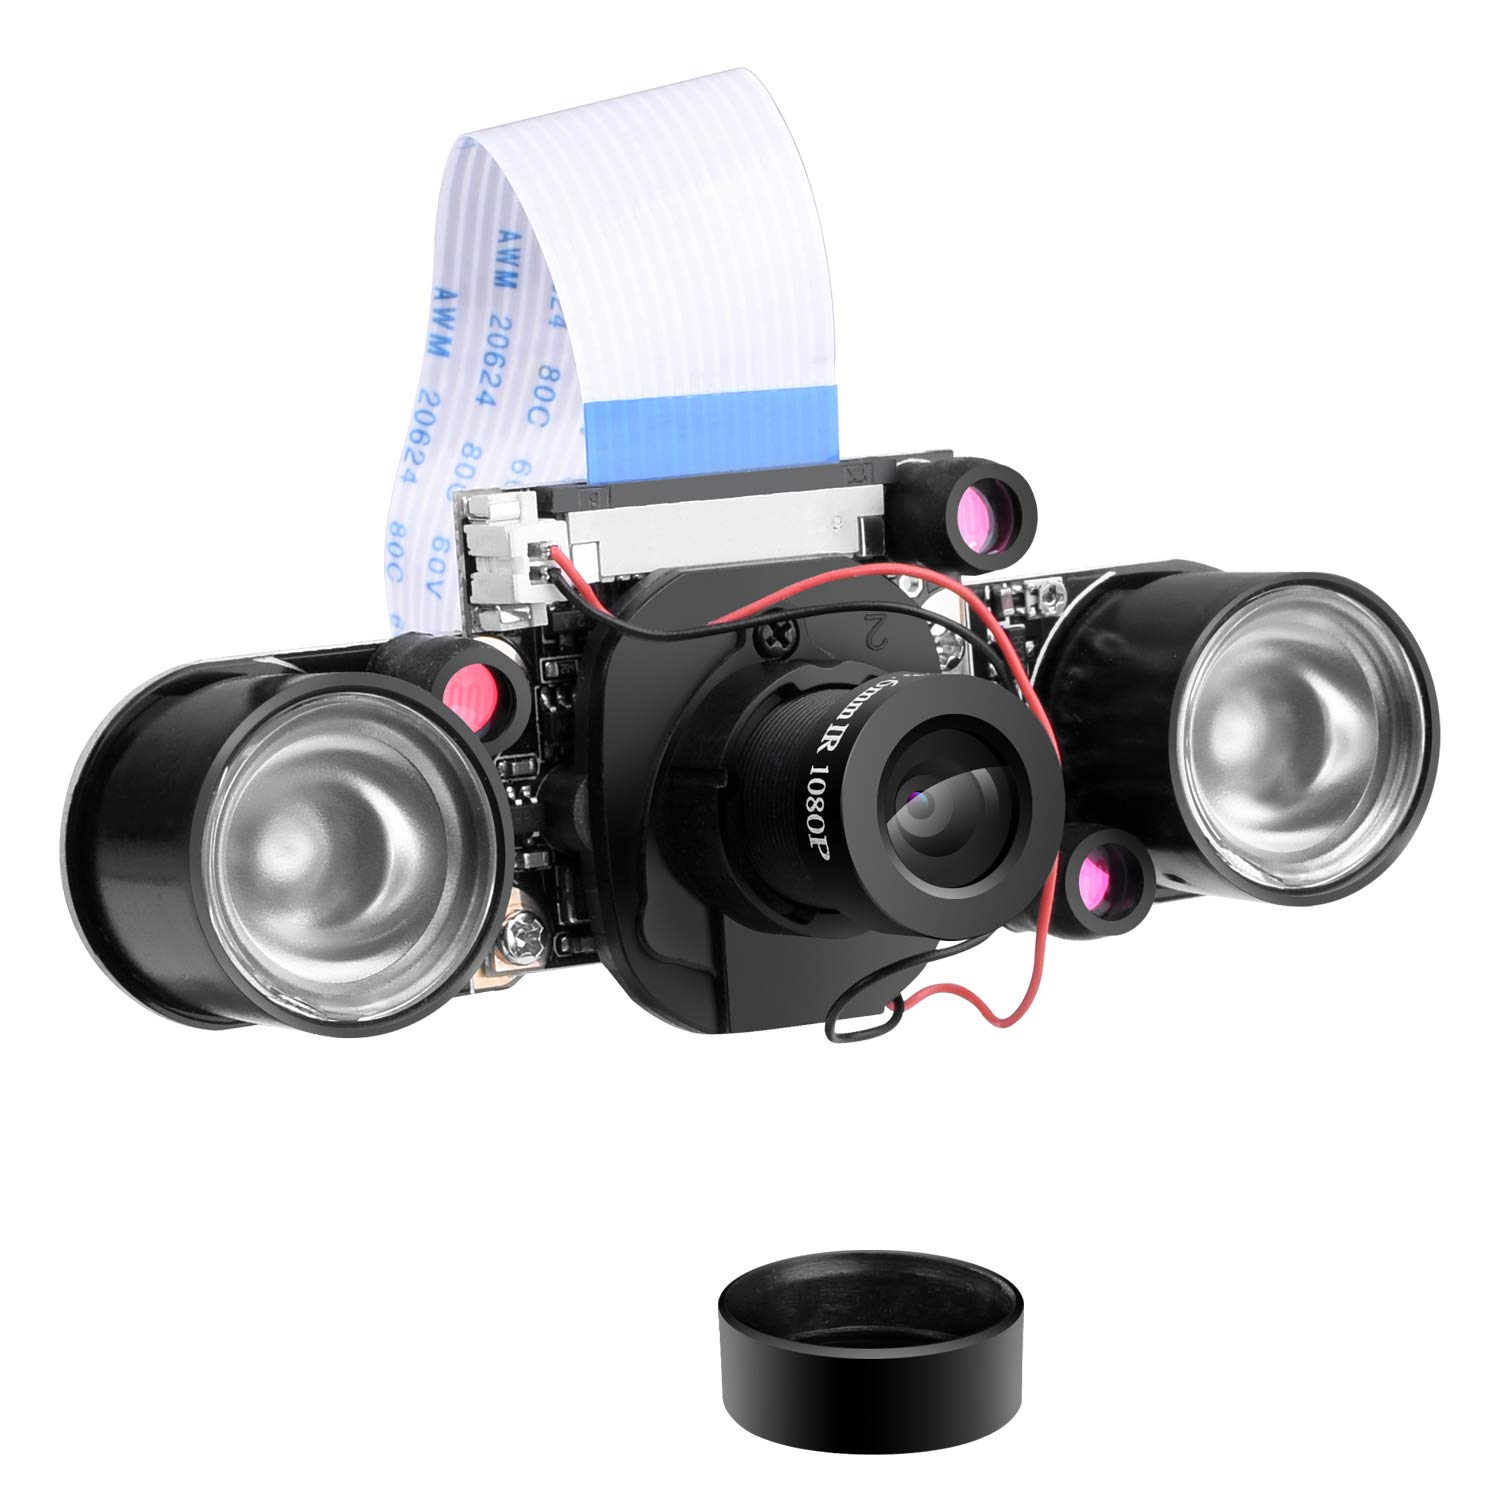
\includegraphics[width=0.8\textwidth]{longrunner.jpg}
    \captionof{figure}{Longruner Kamera Modul}
    \label{fig:rpicam}
\end{minipage}
\vspace{1cm}


Desweiteren wurde für eine mobile Internetverbindung 
der \textit{Huawei E3531 SurfStick} und zu Stromversorgnung
eine Powerbank verwendet.



% https://www.amazon.de/gp/product/B00HSZEY34/ref=ppx_yo_dt_b_asin_title_o00_s00?ie=UTF8&psc=1


\section{Software}


Die Implementierung der Anwendung für den Raspberry Pi wurde in Python.
vorgenommen. Diese ist aufgeteilt in ein \textit{detection.py} 
Script, in welchem die Inferenz implementiert ist und 
einem \textit{connection.py} Script, welches 
für das senden der Daten zuständig ist.
Der Kamera Input Stream ist in einm \textit{main.py} Script implementerit, 
von wo auch die Klassen der detection und connection Scripte, 
dargestellt im Klassendiagramm in Abbildung \ref{fig:class_diagram} 
verwendet werden.


\vspace{1cm}
\begin{figure}[H]
    \centering
    \begin{tikzpicture} 

    
    
            \umlclass{Motion}{ 
              statickBackground : np.array
              }{ 
              + detectMotion() : bool \\
              + resetBackground() : void
            }
        
            \umlclass[y=-4]{InferenceModel}{ 
                string : plugin
                strin : device
                }{ 
                + createExecInferModel() : ExecInferModel
              }
        
            \umlclass[y=-2, x=6]{ExecInferModel}{ 
                shape : ioBlob\\
                detected : array
                }{ 
                + inferFrames() : status \\
                \# status[0] num infered\\
                \# status[1] num detected\\
                \# status[2] num saved\\
                - save() : void
                }
        
    
        \umlclass[x=11, y=-2]{Connection}{ 
            string logindata
            }{ 
            + login() : bool \\
            + connect() : server, port\\
            + send() : bool\\
            + disconnect() : bool\\
            + sendEmail(email, text) : boiol
          }

    
    \end{tikzpicture}
            
    \caption{Klassendiagramm}
    \label{fig:class_diagram}
\end{figure}
\vspace{1cm}

\begin{itemize}
    \item hier beschreibung der klassen
\end{itemize}


Durch geeigneten Implementierung des Applikationsaablaufs, 
sollte eine Möglichkeit gefunden werden, trotz langsamer infere 
zeit, mit dem Faster R-CNN alle Frames in welchen Tiere enthalten 
sind zu inferieren.

Dafür wurde die Annahme gemacht, dass zur Laufzeit der 
Anwendun nicht durchgehen inferiert werden, muss, es also 
Phasenweise sich keine Tiere und 
damit auch keine Bewegung vor der Kamera befinden,

Mithilfe eines Bewegungsmelder, welcher in OpenCV implementerit
wurde und vor der inferenz 
angewendet wurde, ist es möglich nur Frames in denen
Bewegung enthalten ist inferieren zu müssen. 


Input Frames, welche die kamera 
mit einer höheren Fps liefert als 
das Faster R-CNN inferieren kann werden in einer lister/buffer 
zwischengespeichert und nachträglich, wenn keine Bewegung 
mher im Bild detectiert wird inferiert.

Dafür musste der asynchrone Inferenzablauf, wie er typischer 
weise ausgeführt wird \ref{code:async} so abgeändert werden, 
dass er nicht mehr blockierend und damit komplett asynchron 
zu den Input Frames abläuft.

Das Flussdiagramm in Abbildung \ref{fig:flowchart_appl}
zeigt den Gesammtablauf schematisch.

\vspace{1cm}
\begin{figure}[H]
    \centering
    \tikzset{
    desicion/.style={
        diamond,
        draw,
        text width=4em,
        text badly centered,
        inner sep=0pt
    },
    block/.style={
        rectangle,
        draw,
        text width=10em,
        text centered,
        rounded corners
    },
    arrow/.style={
        draw,
        >=latex,
        ->
    }
}


\begin{tikzpicture}
    \node (A) [desicion] {entschei\\dung};
    \node (B) [block, below of=A, node distance=3cm, text width=5em] {bock};
    \node (C) [block, right of=A, node distance=0.5\textwidth] {noch ein\\bock};


    \draw[arrow] (A) --  node [left, fill=white!30] {yes} (B);
    \draw[arrow] (A) -- node [below, near end] {crap} (C); 
    \draw[arrow] (B) -| node [near start, fill=white] {yes} (C);

\end{tikzpicture}
    
    \caption{Main Applikation}
    \label{fig:flowchart_appl}
\end{figure}
\vspace{1cm}

\begin{itemize}
    \item hier flussdiagramm erklären
    \item 
\end{itemize}

bei mehreren inferierten frames ohne bewegung wird 
bewegungsmwlder zurückgesetzt.
erkannet werden nach klassen sortiert gespeichert, 
wobei erkennungen mit höherer genauigkeit ersetzen.

nach N erkennungen wird local gespeicher und ein 
sendrequest an die main gegebe. 
Diese sendet daraufhin alle local 
gespeicherten date an ein verbundenes gerät.

im folgenden werden die einzelnen komponenten
im deteil erklärt.


\subsection*{Inferenz}
Die in Abschnitt \ref{sec:infertime} beschriebene asynchrone 
Inferenz wurde dahingehend abgeändert, dass nun theoretsch belibieg file 
Requests verwendete werden können und für den wait Befehl der 
Timeout auf 0ms gesetzt wurde und so der Ablauf nicht mehr Blockierend 
ist. Dadurch kann die Inferenz unabhängig von der Frequenz der 
von der Kamera erhaltenen Bilder ablaufen.
Auf eine richtige zuordnung der Inferenz ergebnisse zu dem 
jeweiligen verwendeten Frame war zu achten.


\begin{algorithm}[H]
    \caption{Asynchrone Inferenz, ohne Blockierung}
    \begin{algorithmic}
    \WHILE{\TRUE}
    \STATE capture FRAMES
        \FOR{ReqNr in all InferRequests}
            \STATE status \textbf{wait} for ReqNr
            \IF {status == 0}
                \STATE res = ReqNr.output
            \ENDIF
            
            \IF {Buffer != 0}
                \STATE preprocess ReqNr
                \STATE \textbf{statr} ReqNr
            \ENDIF

            \IF{res != NULL}
                \STATE process result
            \ENDIF
        \ENDFOR
    \ENDWHILE
    \end{algorithmic}
\end{algorithm}    




\subsection*{Motion}

Die Bewegungserkennung wurde mithilfe der Library OpenCV implementiert, indem
zu beginn ein Frame als Refernz abgespeichert wurde.
Mit diesem konnten dann alle weiteren Input frames vergleichen werden 
indem der Abstand der einzelnen Pixel werte berechnet und gemittelt wird.
Beträgt dieser mehr als ein bestimmter threshhold wird das als Bewegung 
gewertet.


\subsection*{Connection}

Um eine Verbindung zwischen Raspberry Pi und Pc herzustellen, 
die unabhängig davon ob sich die geräte im selben 
Netzwerk befinden funktioniert, wurde eine Cloud Proxy Verbindung 
implementerit.

Dafür wurde der Dienst \textit{remot3.it} \cite{remoteit} verwendet, 
mit dem es möglich ist ohne Konfiguration des Routers eine
Netzwerkübergreifende Remote Verbindung zum Raspberry Pi herzustellen.

Da die Daten vom Raspberry aus automatisch gesendet werden sollen, 
wurde der Pc als Remote Gerät implementerit un auf dem Raspberry 
eine SSH Verbindung zum Pc hergestellt.


\begin{figure}[H]
    \centering
    \def\svgwidth{0.7\textwidth}
    \input{Bilder/diagram-connect.pdf_tex}
    \caption{}
    \label{}
\end{figure}


Dafür bot remot3.it eine API die es ermöglicht über Get und Post Requests
den Verbindung auf und Abbau zu automatisieren.

Gesendet wurden die Daten dann per SCP Command (Secure Copy Protocol), 
welches die aufgaebaute SSH Verbiindung verwendet.













% \input{Bilder/class_diagramm/class_diagramm.latex}

% \begin{minipage}{0.3\textwidth}
%     \centering
%     \input{Bilder/diagramme/class_detection.tex}    
% \end{minipage}
% \begin{minipage}{0.3\textwidth}
%     \centering
%     \input{Bilder/diagramme/class_connection.tex}
% \end{minipage}
% \begin{minipage}{0.3\textwidth}
%     \centering
%     \input{Bilder/diagramme/class_motion.tex}
% \end{minipage}

% oder

%\input{Bilder/diagramme/detection_package.tex}

% oder 





%Asynchrone inferenz
%https://docs.openvinotoolkit.org/latest/_demos_python_demos_object_detection_demo_ssd_async_README.html

% main
% \begin{algorithm}[H]
%     \caption{Main Program}
%     \begin{algorithmic}

%     %\STATE INIT EXEC_NET, CAM

%     \WHILE{\TRUE}
%         \STATE capture frame
        
%         \IF{frame has motion}
%             \STATE $buffer \leftarrow frmae$
%         \ENDIF

%         \IF{buffer is empty}
%             \STATE disconnect
%         \ENDIF

%         \STATE result = inferFrames (buffer)

%         \FOR{all results}
%             \STATE process results
%             \IF {saved}
%                 \STATE sendRequest = \TRUE
%             \ENDIF
        

%             \IF {no detectoin for 20 times}
%                 \STATE reset motion background
%                 \STATE delete buffer
%                 \IF {connected}
%                     \STATE disconnect
%                 \ENDIF
%             \ENDIF

%         \ENDFOR

%         \IF {send all every minute}
%             \STATE save current detections
%             \STATE sendRequest = \TRUE
%         \ENDIF

%         \IF{sendRequest == \TRUE}
%             \IF{not logged in}
%                 \STATE log in
%             \ENDIF

%             \IF{not connected}
%                 \STATE connect
%             \ENDIF

%             \STATE server, port $\leftarrow$ connection

%             \STATE sendRequest = \FALSE
%             \FOR{all saved images}
%                 \IF{send image $\rightarrow$ server, port}
%                     \STATE delete image
%                 \ELSE
%                     \STATE sendRequest = \TRUE
%                 \ENDIF
%             \ENDFOR

%         \ENDIF
%     \ENDWHILE


%     \end{algorithmic}
% \end{algorithm}



% \newpage

% \begin{center}
%     \rule{0.8\textwidth}{0.4pt}
%     \begin{lstlisting}[language=Python]
%         def infer_frames(Buffer, threshhold):
%             for idx, inferRequest in all inferRequests:
%                 status = inferRequest.wait(0) # nicht blockierend
%                 if status not ready:
%                     continue
                
%                 if idx in currentFrames:
%                     results = inferRequest.output
%                     frame = currentFrames[idx]

%                 if Buffer not empty:
%                     currentFrames[idx] = Buffer.pop()
%                     infer_frame = preprocess(currentFrames[idx])
%                     inferRequest.async_infer(infer_frame)

%                 if results or frame is None:
%                     continue

%                 for obj in all results:
%                     Class, Roi, Proba <- obj
%                     if Proba < threshhold:
%                         continue
                    
%                     coords <- Roi, frame.shape

%                     infered_frame = draw_rect(frame, coords)

%                     if proba > detectedObjects.proba
%                         replace detectedObjects

%                     if number of detections > x:
%                         send(frame)
                    
%     \end{lstlisting}
%     \rule{0.8\textwidth}{0.4pt}        
% \end{center}


% \centering\rule{0.6\textwidth}{0.4pt}
% \begin\centering{lstlisting}[language=Python]
%     def infer_frames():
%         for all requests:
%             do something \textbf{with} request

%             status = request.wait(0)
%             if status == done:
%                 res = requests.output
%                 frame = current[id]
% \end{lstlisting}
% \centering\rule{0.6\textwidth}{0.4pt}




% % inferenz
% \begin{algorithm}[H]
%     \caption{Asynchrone Inferenz}
%     \begin{algorithmic}
%     \WHILE{\TRUE}
%         \STATE capture Frame
%         \IF{Frame has Motion}
%             \STATE Buffer $\leftarrow$ Frame
%         \ENDIF
%         \FOR{$reqId$ = 0 to $reqMax$}
%             \IF {Model.reqests[$reqId$].wait(0)}
%                 \STATE result = Model.reqests[$reqId$].output
%                 \STATE inferedFrames $\leftarrow$ (result, currentFrames[$reqId$])
%                 \IF {Buffer not empty}
%                     \STATE currentFrames[$reqId$] $\leftarrow$ Buffer 
%                     \STATE inFrame = preprocess: currentFrames[$reqId$]
%                     \STATE Model.inferAsync($reqId$, inFrame)
%                 \ENDIF
%             \ENDIF
%         \ENDFOR
%         \RETURN inferedFrames
%     \ENDWHILE
%     \end{algorithmic}
% \end{algorithm}

% wobei die wait Funktion mit Timeout = 0 nicht blockierend ist.

% Dadurch war es möglich trotz langsamerer inferenz zeit als 
% capture zeit, durch zwischenspeichern alle frames zu inferieren, 
% unter der Annahme, das nur zeitweise bewegung erkannt und damit 
% inferiert werden muss.



